% =============================================================================
%  FIGURE + TABLE BLOCKS for main.tex.
%
%  Use figure* (spans both columns) for everything here except where noted.
%  A plain figure at 0.5\textwidth is ~3.4 in, which is what made the tree
%  unreadable: an 12 in figure scaled to a third of its natural size.
%
%  All paths keep the ../../results/... style already in main.tex.
% =============================================================================


% ---- PRIOR -- single column ------------------------------------------------
% The figure carries no title or subtitle; both are in the caption, which is
% what lets it work at \columnwidth.
\begin{figure}[tb]
  \centering
  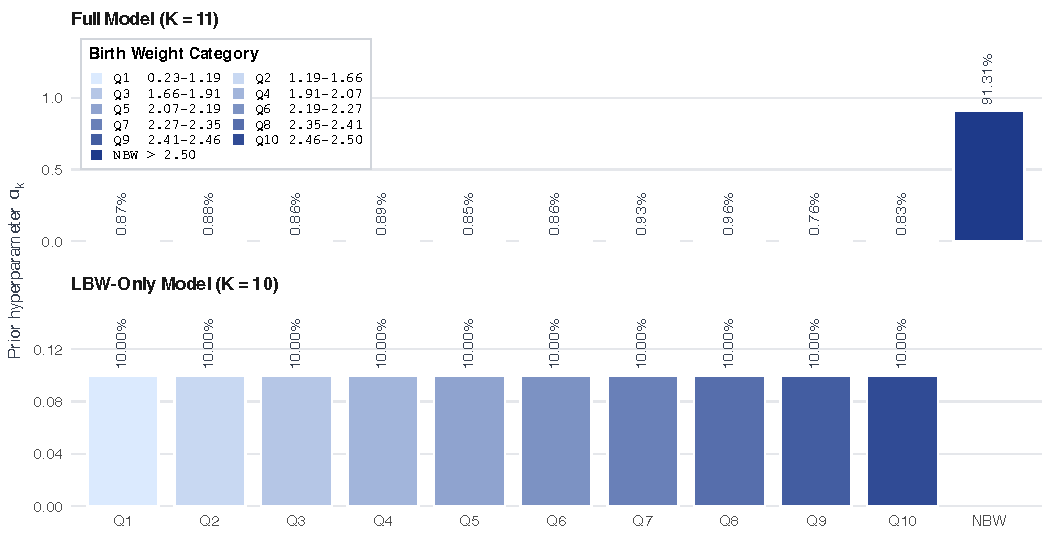
\includegraphics[width=\columnwidth]{../../results/2023-2024/article/informed_prior_2023.pdf}
  \caption[Informed Dirichlet priors from 2023 quantiles]{%
    \textbf{Informed Dirichlet prior hyperparameters.} Bar labels give each
    category's share of the total prior mass and the legend gives each
    category's birth-weight interval in kg, both derived from the 2023
    low-birth-weight distribution. The full model (top) places 91.3\% of its
    prior mass on the normal category (NBW), so the ten LBW deciles are
    compressed on a linear axis and are read from their labels; the LBW-only
    model (bottom) has no NBW category, hence the empty slot. Panels use
    independent $y$ scales.}
  \label{fig:prior}
\end{figure}


% ---- FITTED TREES -- now half a page ---------------------------------------
\begin{figure*}[tb]
  \centering
  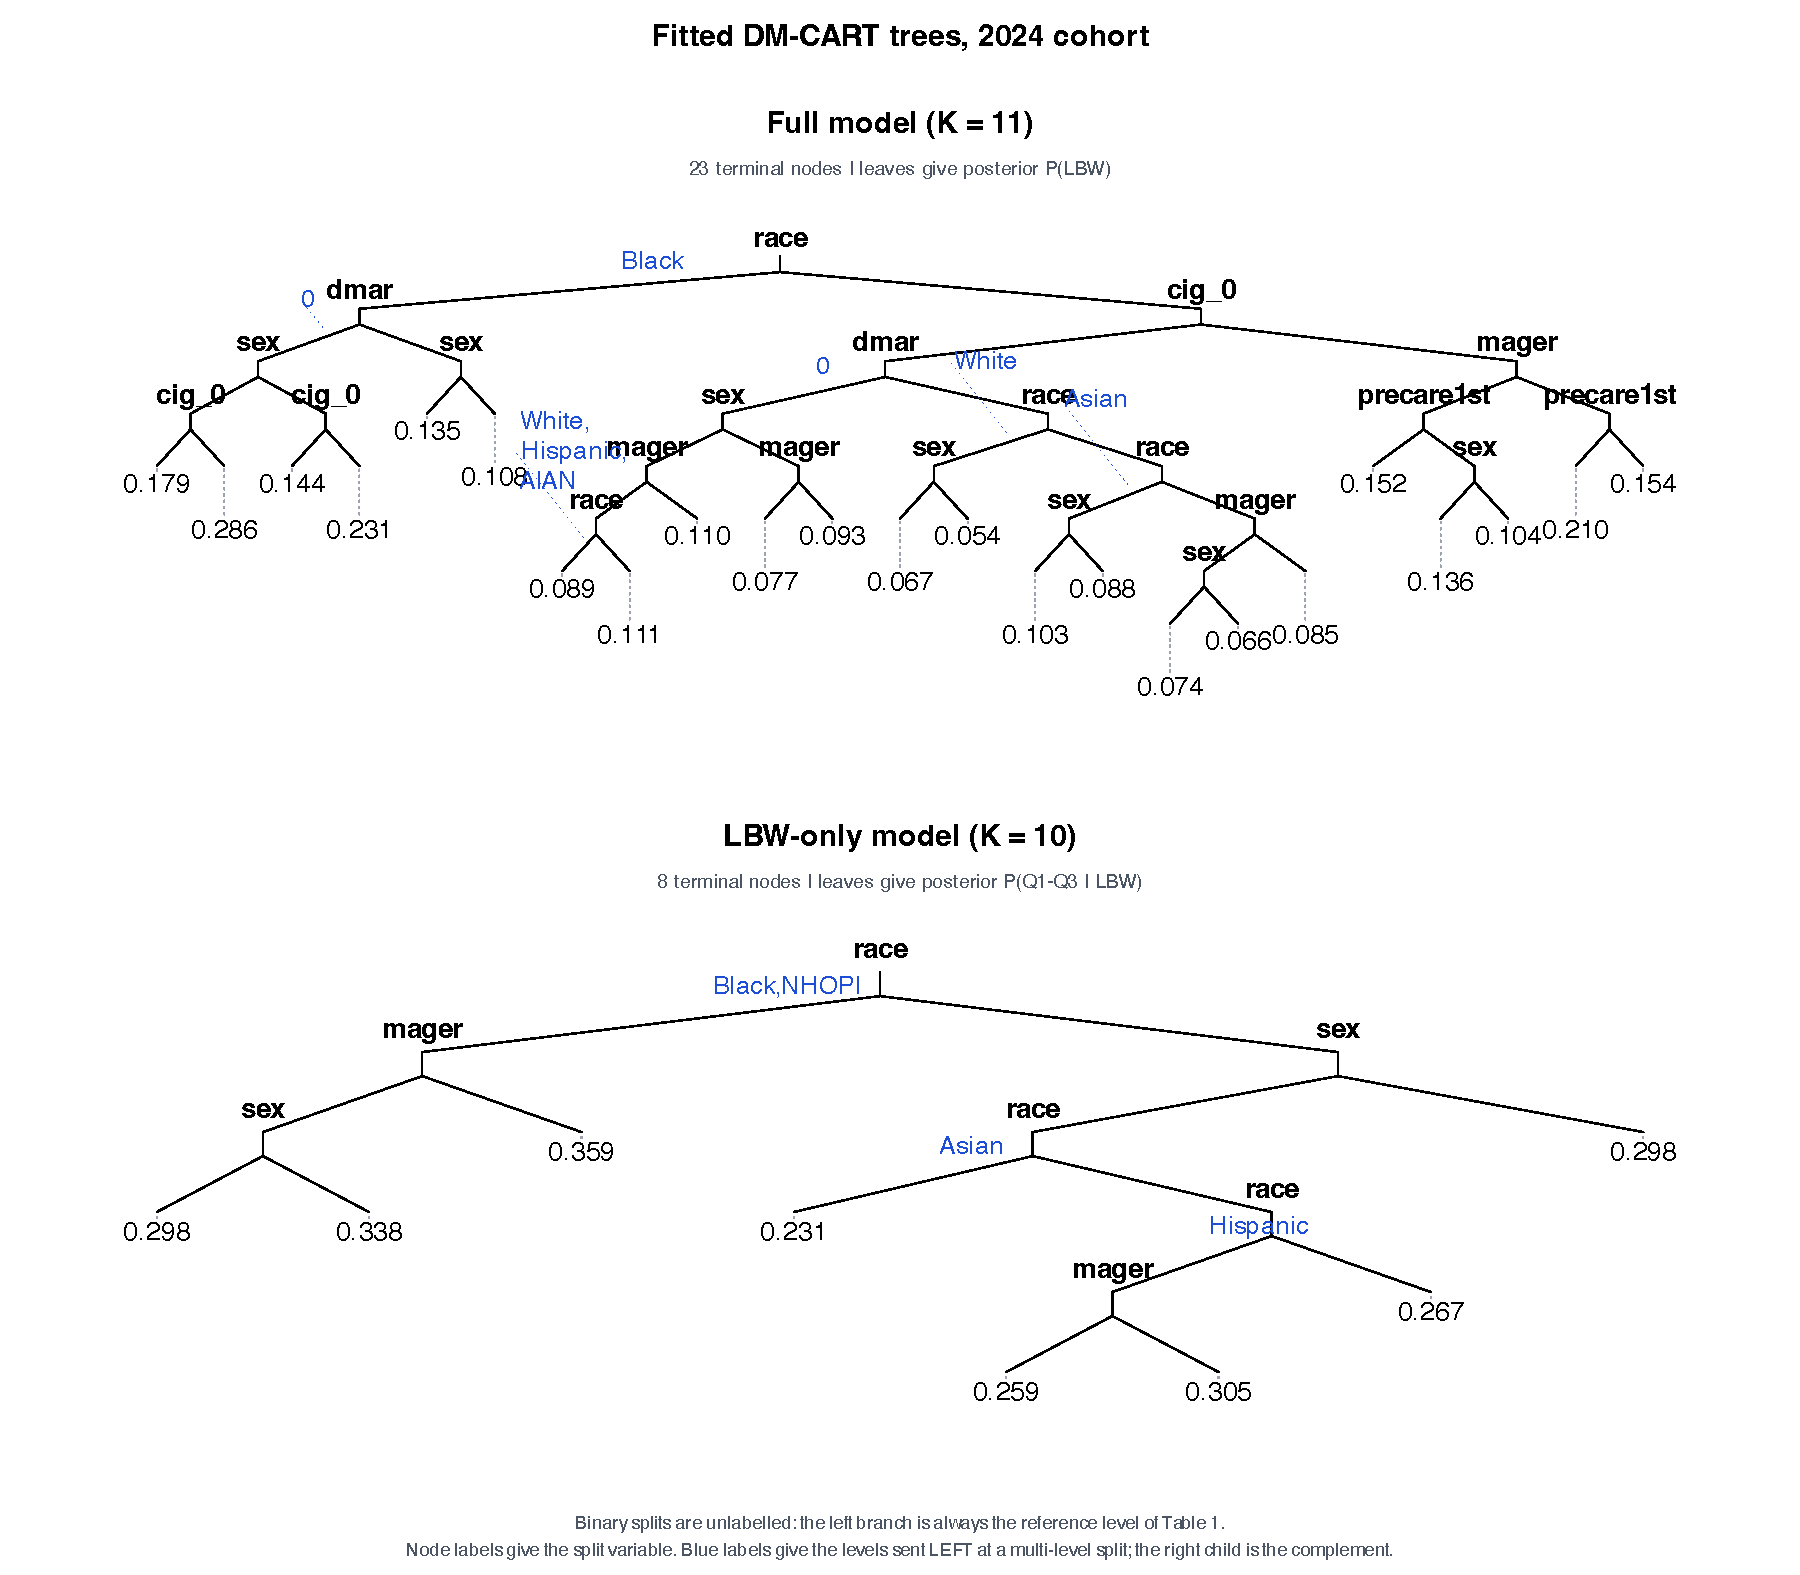
\includegraphics[width=\textwidth]{../../results/2023-2024/article/model_trees_2024.pdf}
  \caption[Fitted DM-CART trees for both model arms]{%
    Fitted DM-CART trees for the 2024 cohort: the full model above, the LBW-only
    model below. Node labels give the split variable. Blue labels give the levels
    sent to the left child at a multi-level split, the right child being the
    complement. Binary splits are unlabelled: the left branch is always the
    reference level ($0$) and the right branch the indicator level ($1$) of
    Table~\ref{tab:vars}. Where a label would overlap the tree it is drawn clear
    of it and joined to its branch by a dotted leader. Terminal nodes give the
    posterior
    risk of the classes routed there --- $P(\mathrm{LBW})$ for the full model and
    $P(Q_1\!-\!Q_3 \mid \mathrm{LBW})$ for the LBW-only model, in which every
    category is by construction an LBW category, so the two panels are on
    different scales. Both trees select maternal race at the root.}
  \label{fig:model-trees}
\end{figure*}


% ---- TREE GROWTH BY DEPTH ---------------------------------------------------
\begin{figure*}[tb]
  \centering
  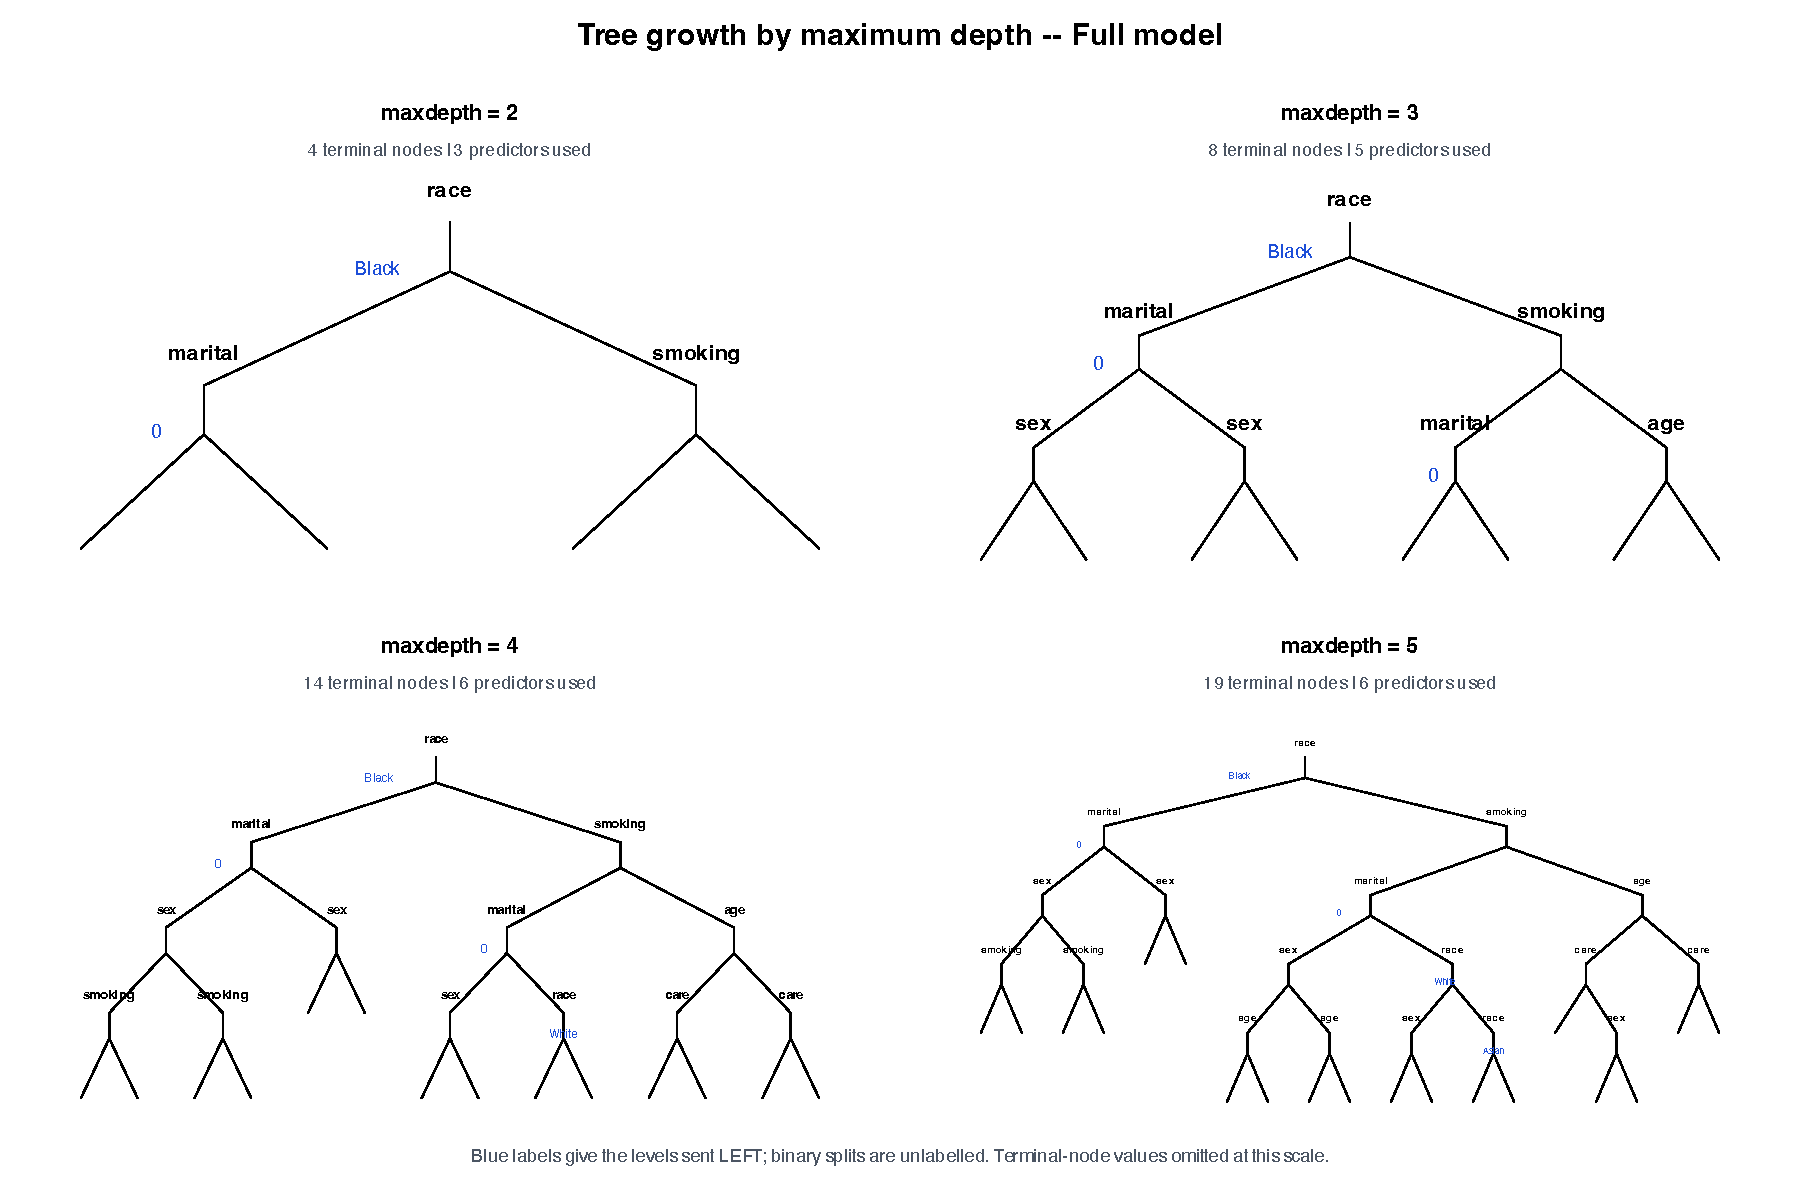
\includegraphics[width=\textwidth]{../../results/2023-2024/article/depth_growth_full_2024.pdf}
  \caption[Tree growth by maximum depth]{%
    Structure of the full model at maximum depths 2--5, showing which predictors
    enter as the tree is allowed to grow: three at depth~2, five at depth~3, and
    six from depth~4 onward. Maternal education never enters at any depth.
    Terminal-node values are omitted at this scale and are reported in
    Table~\ref{tab:depth}. Node labels are abbreviated: \texttt{marr} marital
    status, \texttt{age} maternal age $>33$, \texttt{educ} high school completed,
    \texttt{care} first-trimester prenatal care, \texttt{smoke} any pre-pregnancy
    smoking.}
  \label{fig:depth-growth}
\end{figure*}


% ---- CATEGORY PROBABILITIES FOR THE EXTREME CLASSES -------------------------
% NOTE: this is the figure that shows the actual probabilities with error bars.
\begin{figure*}[tb]
  \centering
  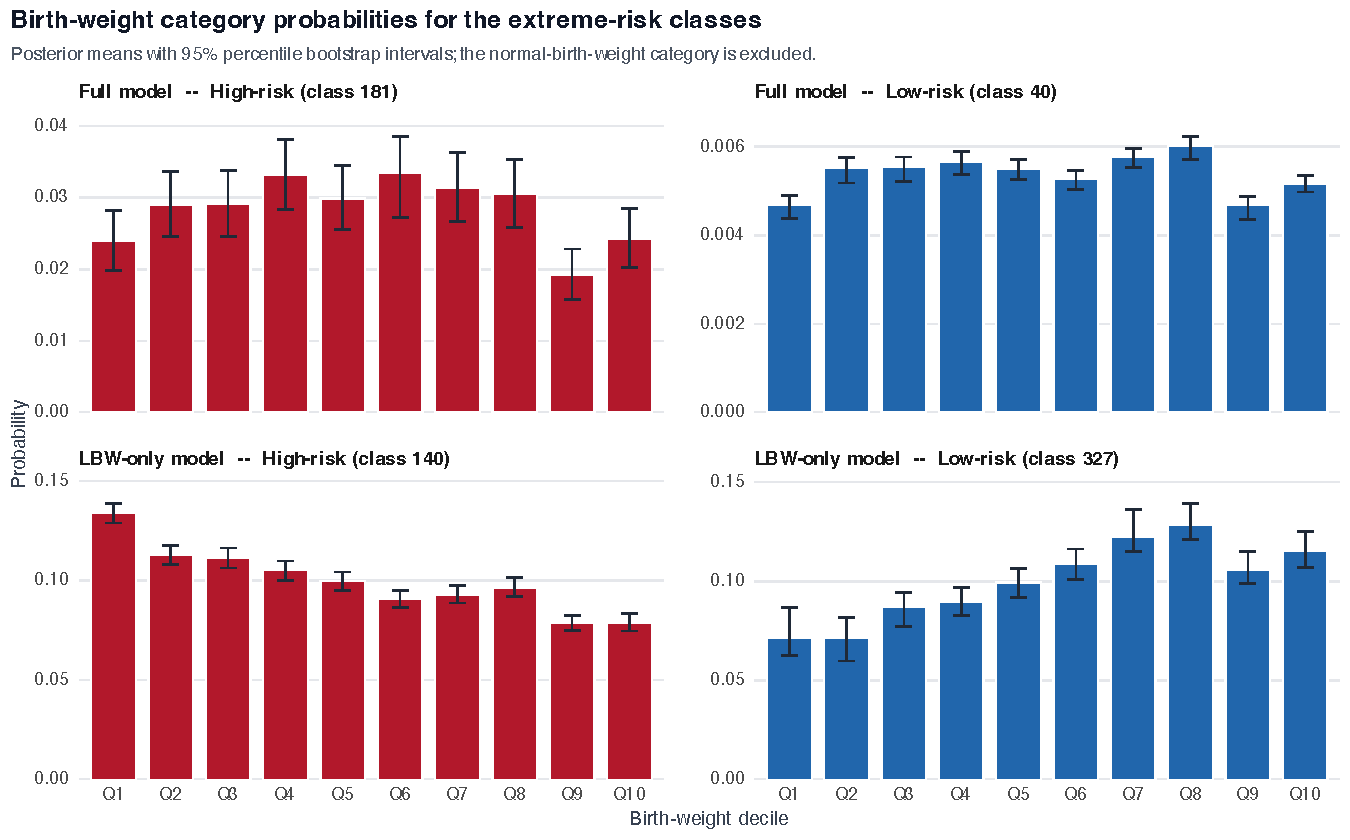
\includegraphics[width=0.94\textwidth]{../../results/2023-2024/article/risk_category_profiles_2024.pdf}
  \caption[Category probabilities for the extreme-risk classes]{%
    Posterior probability of each low-birth-weight decile for the highest- and
    lowest-risk class of each model arm, with 95\% percentile bootstrap intervals
    from the 10{,}000-tree ensemble. The normal-birth-weight category is excluded
    so the shape within the LBW region is visible; panels use independent $y$
    scales. In the LBW-only model the highest-risk class concentrates mass in the
    smallest deciles while the lowest-risk class shifts toward the largest,
    a severity gradient the binary LBW indicator cannot express.}
  \label{fig:risk-profile}
\end{figure*}


% ---- RISK LANDSCAPE -- single column, stacked -------------------------------
\begin{figure}[tb]
  \centering
  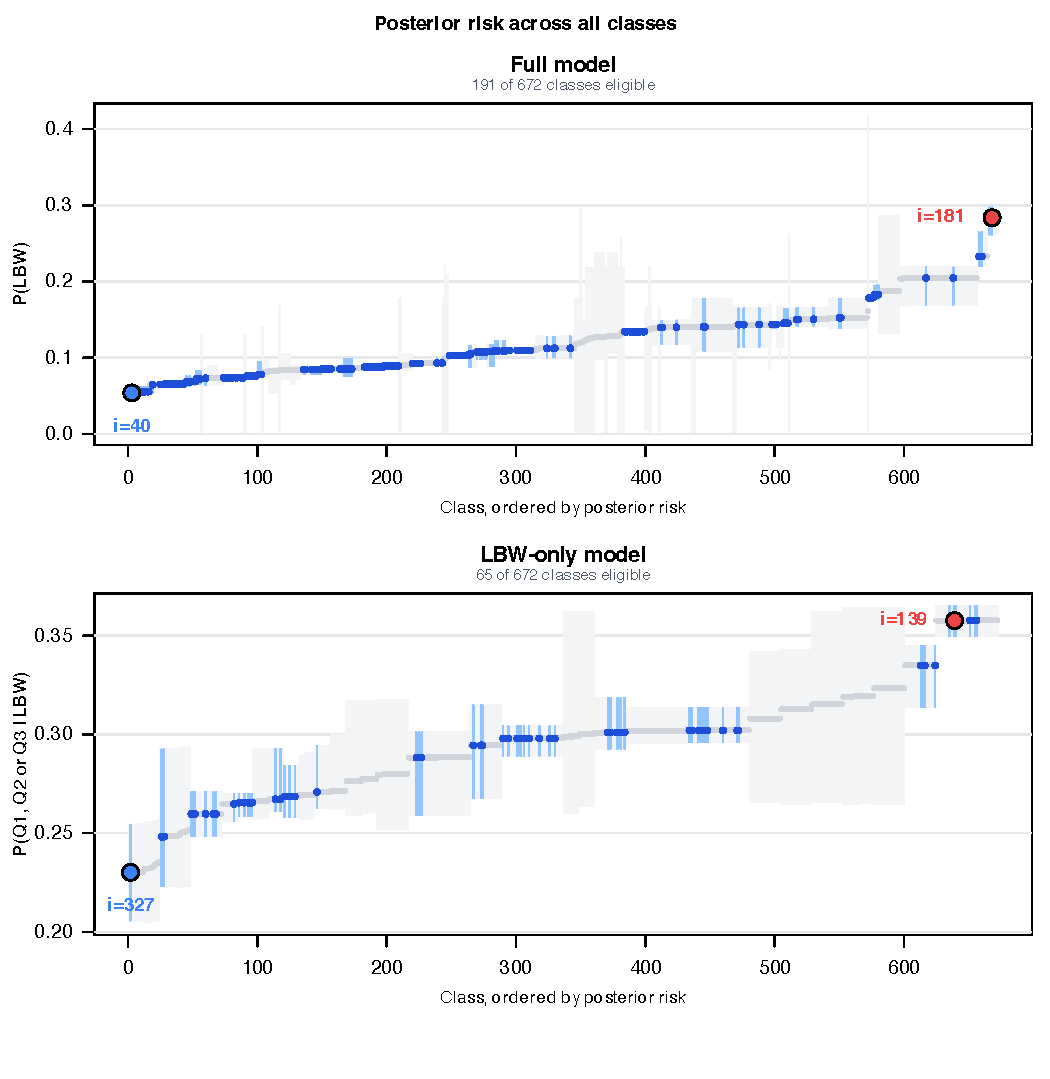
\includegraphics[width=\columnwidth]{../../results/2023-2024/article/risk_profile_ranking_2024.pdf}
  \caption[Posterior risk across all classes]{%
    Posterior risk for all 672 maternal-infant classes, the full model above and
    the LBW-only model below, ordered by risk with 95\% percentile bootstrap
    intervals. Filled points are classes meeting the support threshold of
    1{,}000 observed births (191 of 672 in the full model, 65 in the LBW-only
    model); hollow grey points fall below it and are excluded from the ranking,
    but are shown so the extent of the filter is visible. Red and blue mark the
    highest- and lowest-risk class in each arm. Note the two arms use different
    risk scores and therefore different $y$ scales.}
  \label{fig:risk-landscape}
\end{figure}


% ---- COMMONALITIES AMONG THE EXTREME PROFILES -------------------------------
% Auto-generated by visual.R; \input rather than paste, so it stays in sync.
% Auto-generated by visual.R -- do not edit by hand.
\begin{table}[tb]
\centering\footnotesize
\caption[Shared features of the extreme-risk classes]{Shared features of the ten highest- and ten lowest-risk classes. Each cell gives the level carried by most of the ten and how many carry it; \textbf{bold} marks a level shared by all ten. Classes with fewer than 1,000 observed births are excluded.}
\label{tab:commonality}
\begin{tabular}{@{}lcc@{}}
\toprule
\textbf{Predictor} & \textbf{Highest 10} & \textbf{Lowest 10} \\
\midrule
\multicolumn{3}{@{}l@{}}{\textit{Full model}} \\
\quad \texttt{sex} & 0 (7/10) & \textbf{1} (10/10) \\
\quad \texttt{dmar} & \textbf{0} (10/10) & 1 (6/10) \\
\quad \texttt{mager} & 1 (6/10) & 0 (6/10) \\
\quad \texttt{meduc} & 1 (8/10) & 1 (7/10) \\
\quad \texttt{precare1st} & 0 (6/10) & 1 (6/10) \\
\quad \texttt{cig\_0} & 1 (6/10) & \textbf{0} (10/10) \\
\quad \texttt{race} & Black (8/10) & \textbf{White} (10/10) \\
\addlinespace
\multicolumn{3}{@{}l@{}}{\textit{LBW-only model}} \\
\quad \texttt{sex} & 1 (7/10) & \textbf{0} (10/10) \\
\quad \texttt{dmar} & 0 (7/10) & 0 (4/10) \\
\quad \texttt{mager} & 1 (6/10) & 0 (8/10) \\
\quad \texttt{meduc} & 1 (9/10) & 1 (8/10) \\
\quad \texttt{precare1st} & 1 (6/10) & 1 (7/10) \\
\quad \texttt{cig\_0} & \textbf{0} (10/10) & \textbf{0} (10/10) \\
\quad \texttt{race} & \textbf{Black} (10/10) & Hispanic (7/10) \\
\bottomrule
\end{tabular}
\end{table}


% Optional companion figure -- the same analysis as a shaded profile grid.
% Use EITHER this or the table above; both say the same thing.
%
% \begin{figure*}[tb]
%   \centering
%   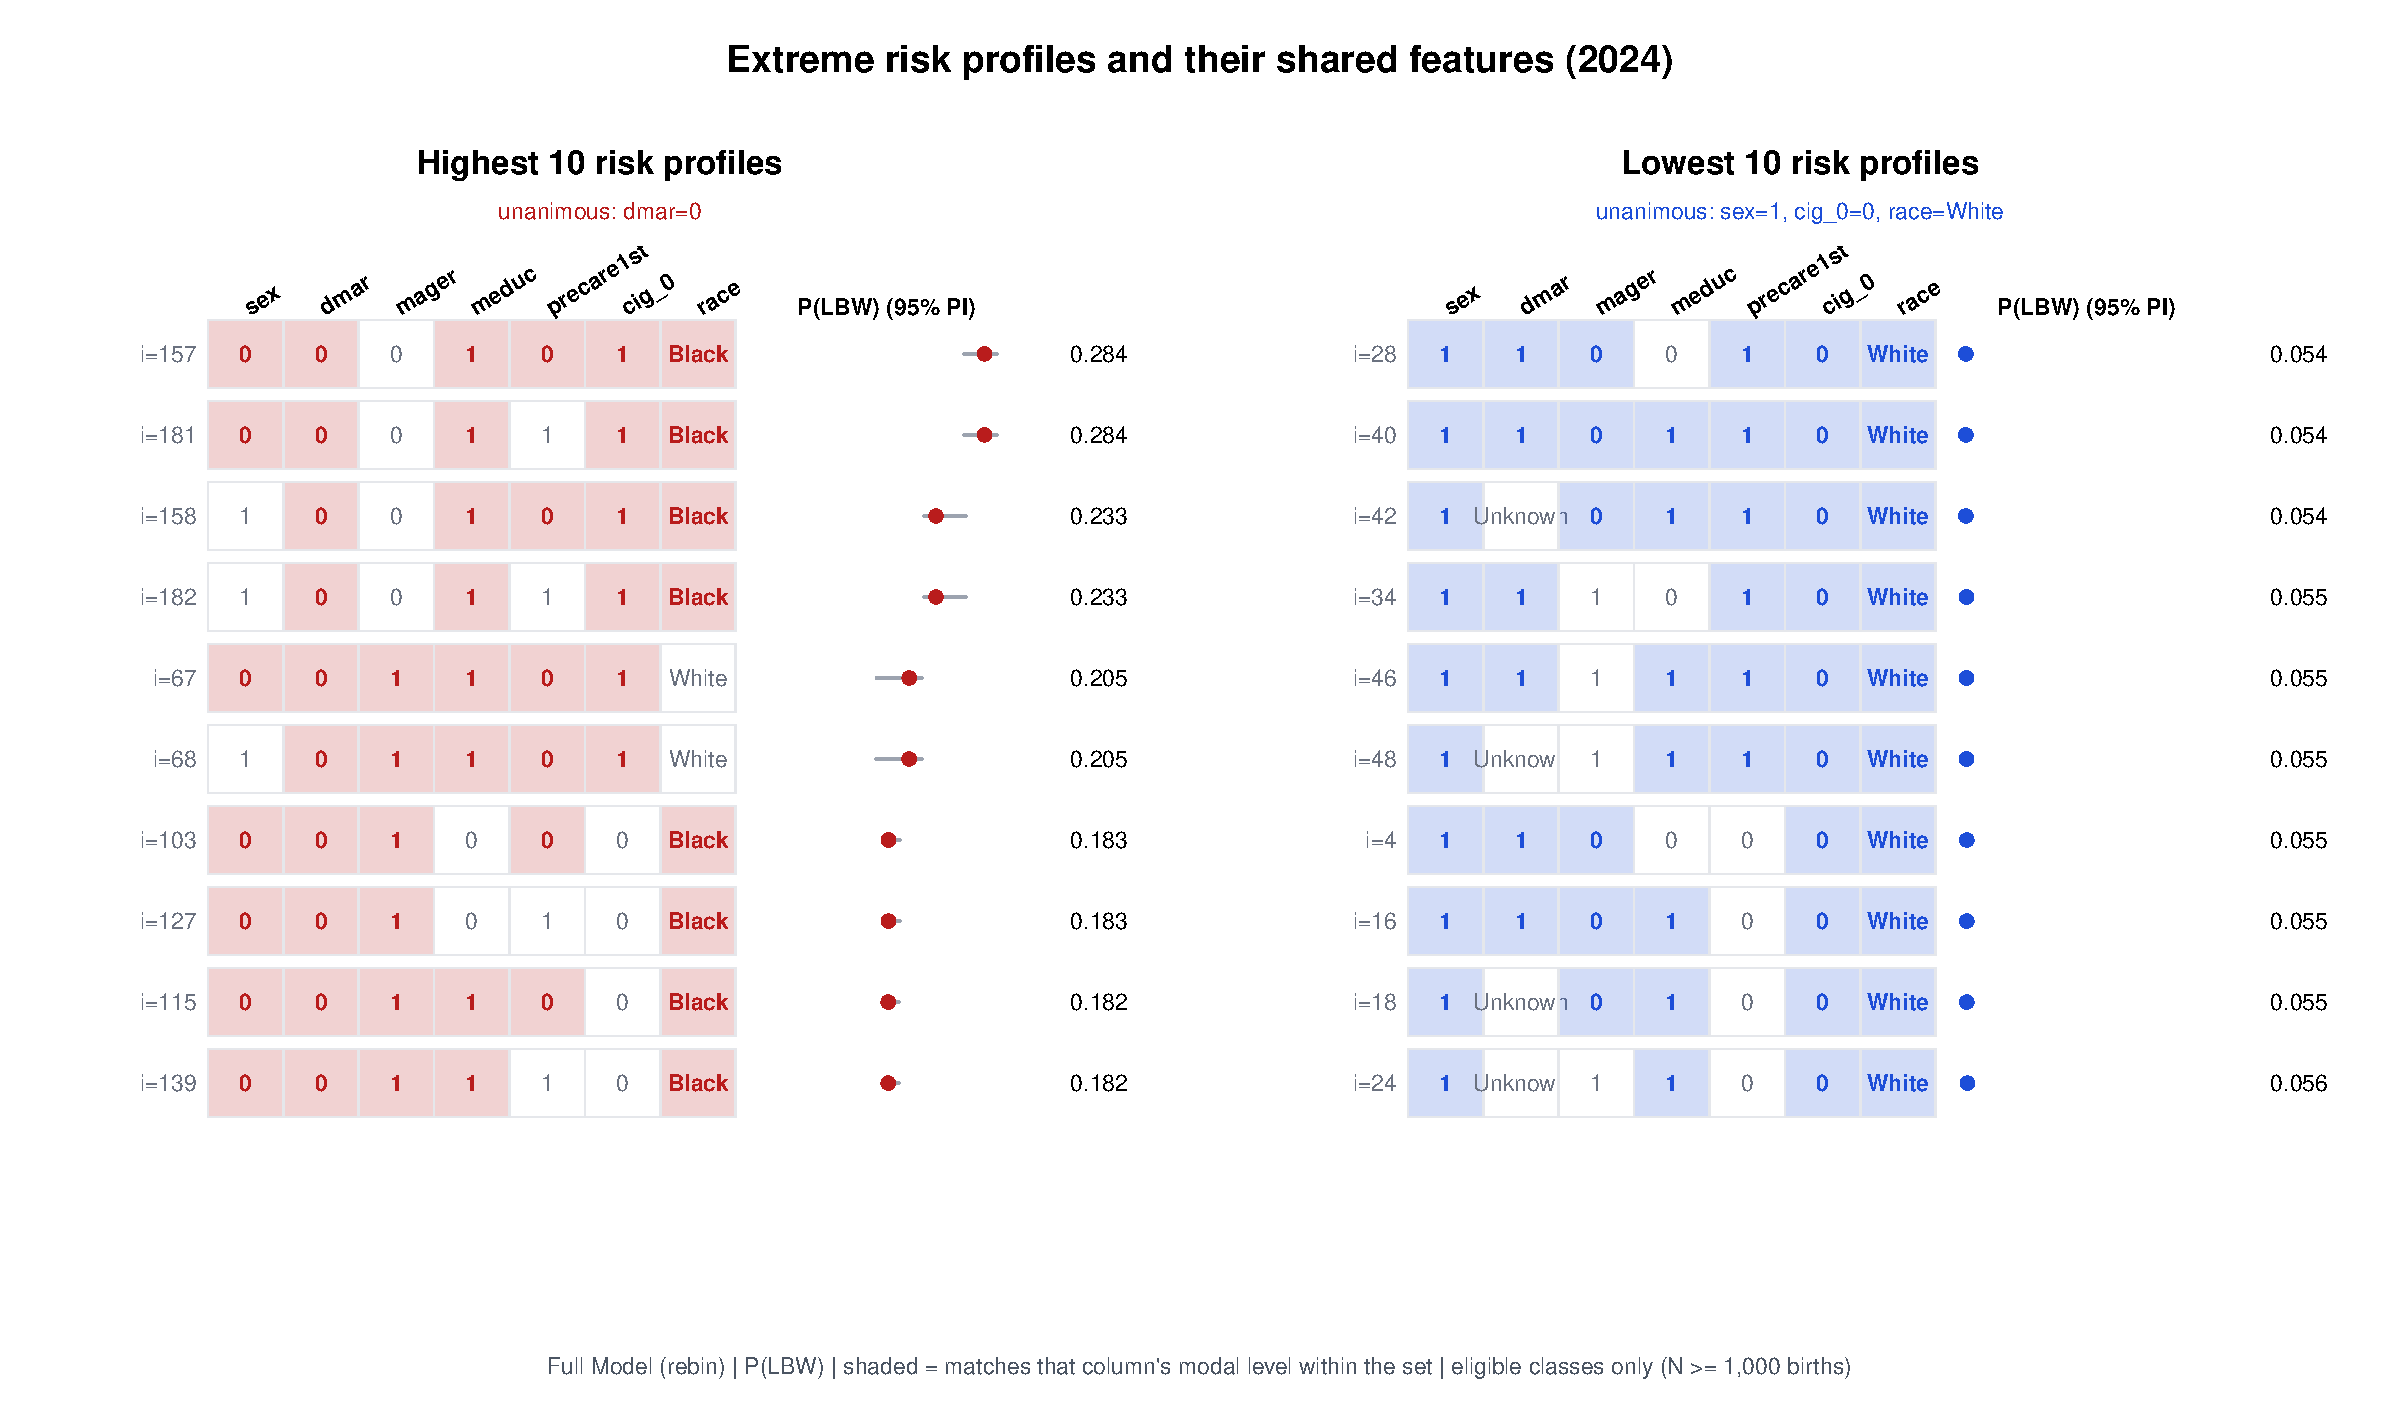
\includegraphics[width=\textwidth]{../../results/2023-2024/article/risk_extremes_profiles_full_2024.pdf}
%   \caption[Extreme risk profiles and their shared features]{%
%     The ten highest- and ten lowest-risk classes of the full model. Rows are
%     profiles ordered by risk; columns are the seven predictors, with a cell
%     shaded when its level matches that column's modal level within the set, so a
%     fully shaded column marks a feature shared by all ten. Posterior
%     $P(\mathrm{LBW})$ with its 95\% percentile interval is shown at right.}
%   \label{fig:extremes}
% \end{figure*}
